\documentclass{paper}

\usepackage{graphicx}
\usepackage{placeins}
\usepackage[utf8]{inputenc}
\usepackage{listings}
\usepackage{hyperref}
\usepackage{xcolor}
\usepackage{mathtools}

\DeclarePairedDelimiter{\ceil}{\lceil}{\rceil}

\definecolor{darkgreen}{RGB}{50,200,50}
\definecolor{verylightgray}{gray}{0.85}
\definecolor{goldenbrown}{rgb}{0.558215, 0.0, 0.135316}

\lstdefinelanguage{solidity}
{
	keywords={uint256, bytes32, mapping, address, uint40, bool, uint32, msg, sender, false, true},
	keywordstyle=\color{blue},
	keywords=[2]{pragma, contract, event, enum, struct, function, return, private, public, constant, returns, var, for, !, if, break, continue, throw, &&, ||, else, =, ==, <, >, <=, >=},
	keywordstyle=[2]\color{magenta},
	comment=[l]{//},
	commentstyle=\color{darkgreen},
	numbers=left,
	extendedchars=false,
	morestring=[b]",
	stringstyle=\color{goldenbrown},
	breaklines=true,
	backgroundcolor=\color{verylightgray},
	basicstyle=\linespread{1}\ttfamily\footnotesize
}

\title{Consensus in declarative process models using distributed smart-contracts}
\author{Mikkel Gaub, \\ Trondúr Høgnason, \\ Malthe Ettrup Kirkbro, \\ \& Mads Frederik Madsen }
\date{}

\begin{document}
	\begin{titlepage}
		\maketitle		
		\hspace{-18pt}
		\textit{May 15, 2017}
		\vspace{\fill}
		\section*{Abstract}
		This paper investigates how efficently declarative process models can be implemented using distributed smart-contracts, more concretely the Dynamic Condition Response (DCR) engine will be implemented on the Ethereum platform, with a focus on minimizing the cost of running such an engine.
		\thispagestyle{empty}
	\end{titlepage}
	\clearpage

	\pagenumbering{arabic}
	\setcounter{page}{1}

	\tableofcontents
	\pagebreak

	\section{Introduction}

	\section{DCR}

	Exclusion of Spawn relation.

	\section{Ethereum}

		\subsection{Blockchain}

		\subsection{Ethereum Virtual Machine}

		\subsection{Currency}

	\section{Implementation requirements}

	All of the proposed solutions will contain the following features:
	\begin{itemize}
		\item Creation of a workflow
		\item Execution of an activity
		\item Execution rights on the level of a user and on the level of a group
		\item Visibility?
	\end{itemize}


	\section{Multi-contract implementation}

	As the gas costs of ethereum are largely dominated by the price of creating a contract, creating a contract for each activity seems unfeasible and also has security concerns related to it which will be covered later...

	The first proposed solution is creating a contract for each workflow...

	\section{Mono-contract implementation}

	The second proposed solution is creating a single contract which controls all workflows...

	\section{Comparison}
	In order to compare the solutions to each other, a simple workflow has been created modelling each of the five relations...

	\begin{description}
		\item[Contract creation]
		\item[Successful execution] ...
		\item[Failed execution] ... 
	\end{description}

	\section{Optimizations}

		\subsection{Bitfields}

		\subsection{Incoming/Outgoing}

		\subsection{etc.}


	\section{Discussion}

	\section{Further features}

		\subsection{External relations}

		\subsection{Workflow changes}

		\subsection{External contract conditions}

	\section{Vulnerabilities}

		\subsection{External relations attack}

		\subsection{Workflow updating attack}

	\section{Conclusion}

	\pagebreak
	\addcontentsline{toc}{section}{References}	
	\begin{thebibliography}{99}

		\bibitem{test}
		Dr. Bib Example,
		\textit{How to bib},
		Penguin publishing,
		1994

	\end{thebibliography}

	\appendix

	\section{Gas prices}

		\begin{tabular}{| l | l | l |}
			\hline
			Name 				& Value 	& Description \\ \hline
			$G_{zero}$ 			& 0 		& Nothing paid for operations of set $W_{zero}$. \\ \hline
			$G_{base}$ 			& 2 		& Amount of gas to pay for operations of the set $W_{base}$. \\ \hline
			$G_{verylow}$ 		& 3 		& Amount of gas to pay for operations of the set $W_{verylow}$. \\ \hline
			$G_{low}$ 			& 5 		& Amount of gas to pay for operations of the set $W_{low}$. \\ \hline
			$G_{mid}$ 			& 8 		& Amount of gas to pay for operations of the set $W_{mid}$. \\ \hline
			$G_{high}$ 			& 10 		& Amount of gas to pay for operations of the set $W_{high}$. \\ \hline
			$G_{extcode}$ 		& 700 		& Amount of gas to pay for operations of the set $W_{extcode}$. \\ \hline
			$G_{balance}$ 		& 400 		& Amount of gas to pay for a BALANCE operation. \\ \hline
			$G_{sload}$ 		& 200 		& Paid for a SLOAD operation. \\ \hline
			$G_{jumpdest}$ 		& 1 		& Paid for a JUMPDEST operation. \\ \hline
			$G_{sset}$ 			& 20000 	& Paid for an SSTORE operation when the storage value is set to non-zero from zero. \\ \hline
			$G_{sreset}$ 		& 5000 		& Paid for an SSTORE operation when the storage value's zeroness remains unchanged or is set to zero. \\ \hline
			$R_{sclear}$ 		& 15000		& Refund given (added into refund counter) when the storage value is set to zero from non-zero. \\ \hline
			$R_{suicide}$ 		& 24000 	& Refund given (added into refund counter) for suiciding an account. \\ \hline
			$G_{suicide}$ 		& 5000 		& Amount of gas to pay for a SUICIDE operation. \\ \hline
			$G_{create}$ 		& 32000		& Paid for a CREATE operation. \\ \hline
			$G_{codedeposit}$ 	& 200 		& Paid per byte for a CREATE operation to succeed in placing code into state. \\ \hline
			$G_{call}$ 			& 700		& Paid for a CALL operation. \\ \hline
			$G_{callvalue}$ 	& 9000		& Paid for a non-zero value transfer as part of the CALL operation. \\ \hline
			$G_{calstipend}$ 	& 2300		& A stipend for the called contract subtracted from $G_{callvalue}$ for a non-zero value transfer. \\ \hline
			$G_{newaccount}$ 	& 25000		& Paid for a CALL or SUICIDE operation which creates an account. \\ \hline
			$G_{exp}$ 			& 10 		& Partial payment for an EXP operation \\ \hline
			$G_{expbyte}$ 		& 10		& Partial payment when multiplied by $\ceil{log_{256}(exponent)}$  for the EXP operation. 	 \\ \hline
			$G_{memory}$ 		& 3			& Paid for every additional word when expanding memory. \\ \hline
			$G_{txcreate}$ 		& 32000		& Paid by all contract-creating transactions after the Homestead transition. \\ \hline
			$G_{txdatazero}$ 	& 4 		& Paid for every zero byte of data or code for a transaction. \\ \hline
			$G_{txdatanonzero}$ & 68		& Paid for every non-zero byte of data or code for a transaction. \\ \hline
			$G_{transaction}$ 	& 21000		& Paid for every transaction. \\ \hline
			$G_{log}$ 			& 375 		& Partial payment for a LOG operation. \\ \hline
			$G_{logdata}$ 		& 8			& Paid for each byte in a LOG operation's data. \\ \hline
			$G_{logtopic}$ 		& 375		& Paid for each topic of a LOG operation. \\ \hline
			$G_{sha3}$ 			& 30		& Paid for each SHA3 operation. \\ \hline
			$G_{sha3word}$ 		& 6			& Paid for each word (rounded up) for input data to a SHA3 operation. \\ \hline
			$G_{copy}$ 			& 3			& Partial payment for *COPY operations, multiplied by words copied, rounded up. \\ \hline
			$G_{blockhash}$ 	& 20		& Payment for BLOCKHASH operation. \\ 
			\hline
		\end{tabular}

		\subsection{Instruction sets}
		\begin{description}
			\item[$W_{zero}$] \{STOP, RETURN\}
			\item[$W_{base}$] \{ADDRESS, ORIGIN, CALLER, CALLVALUE, CALLDATASIZE, CODESIZE, GASPRICE, COINBASE, TIMESTAMP, NUMBER, DIFFICULTY, GASLIMIT, POP, PC, MSIZE, GAS \}
			\item[$W_{verylow}$] \{ADD, SUB, NOT, LT, GT, SLT, SGT, EQ, ISZERO, AND, OR, XOR, BYTE, CALLDATALOAD, MLOAD, MSTORE, MSTORES, PUSH*, DUP*, SWAP*\}
			\item[$W_{low}$] \{MUL, DIV, SDIV, MOD, SMOD, SIGNEXTEND\}
			\item[$W_{mid}$] \{ADDMOD, MULMOD, JUMP\}
			\item[$W_{high}$] \{JUMPI\}
			\item[$W_{extcode}$] \{EXTCODESIZE\}			
		\end{description}

	\section{Test workflow}

		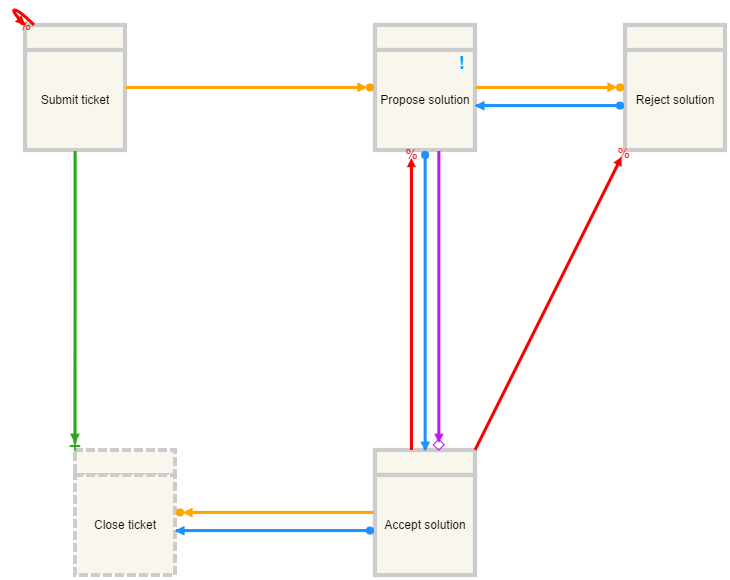
\includegraphics[scale=0.45]{figures/ExampleWorkflow.png}

	\section{Multi-contract}

		\subsection{Code}

			\lstinputlisting[language=solidity]{../contracts/workflow.sol}

		\subsection{Costs}

			\begin{tabular}{| l | l |}
				\hline
				Action & Cost (gas) \\ \hline
				Contract creation & 0 \\
				\hline
			\end{tabular}

	\section{Mono-contract}

		\subsection{Code}

			\lstinputlisting[language=solidity]{../contracts/monolith.sol}

		\subsection{Costs}

			\begin{tabular}{| l | l |}
				\hline
				Action & Cost (gas) \\ \hline
				Contract creation & 0 \\
				\hline
			\end{tabular}

\end{document}